\protect\hyperlink{main-nav}{≡} \protect\hyperlink{close-nav}{×}

\hypertarget{chapter-4-functions-of-two-variables}{%
\section{Chapter 4: Functions of Two
Variables}\label{chapter-4-functions-of-two-variables}}

\hypertarget{pre-calculus-idea-topological-maps}{%
\subsection{Pre-Calculus Idea -- Topological
Maps}\label{pre-calculus-idea-topological-maps}}

If you've ever hiked, you have probably seen a topographical map. Here
is part of a topographic map of Stowe, Vermont.

\begin{figure}
\centering
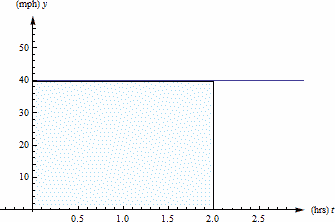
\includegraphics{images/image001.png}
\caption{(Figure courtesy of United States Geological Survey and
\url{http://en.wikipedia.org/wiki/File:Topographic_map_example.png}.)}
\end{figure}

Points with the same elevation are connected with curves, so you can
read not only your east-west and your north-south location, but also
your elevation. You may have also seen weather maps that use the same
principle -- points with the same temperature are connected with curves
(isotherms), or points with the same atmospheric pressure are connected
with curves (isobars). These maps let you read not only a places
location but also its temperature or atmospheric pressure.

In this chapter, we will use that same idea to make graphs of functions
of two variables.

\hypertarget{section-4.1-functions-of-two-variables}{%
\section{Section 4.1: Functions of Two
Variables}\label{section-4.1-functions-of-two-variables}}

\hypertarget{introduction}{%
\subsection{Introduction}\label{introduction}}

Real life is rarely as simple as one input / one output. Many
relationships depend on lots of variables. Examples:

\begin{itemize}
\tightlist
\item
  If I put a deposit into an interest-bearing account and let it sit,
  the amount I have at the end of 3 years depends on
  \textbackslash{}(P\textbackslash{}) (how much my initial deposit is),
  \textbackslash{}(r\textbackslash{}) (the annual interest rate), and
  \textbackslash{}(n\textbackslash{}) (the number of compoundings per
  year).
\item
  The air resistance on a wing in a wind tunnel depends on the shape of
  the wing, the speed of the wind, the wing's orientation (pitch, yaw,
  and roll), plus a myriad of other things that I can't begin to
  describe.
\item
  The amount of your television cable bill depends on which basic rate
  structure you have chosen and how many pay-per-view movies you
  ordered.
\end{itemize}

Since the real world is so complicated, we want to extend our calculus
ideas to functions of several variables.

\hypertarget{functions-of-two-variables}{%
\subsection{Functions of Two
Variables}\label{functions-of-two-variables}}

If \textbackslash{}( x\_1, x\_2, x\_3, \textbackslash{}dots, x\_n
\textbackslash{}) are real numbers, then \textbackslash{}( (x\_1, x\_2,
x\_3, \textbackslash{}dots, x\_n) \textbackslash{}) is called an
\textbackslash{}(n\textbackslash{})-tuple. This is an extension of
ordered pairs and triples. A function of n variables is a function whose
domain is some set of \textbackslash{}(n\textbackslash{})-tuples and
whose range is some set of real numbers.

For much of what we do here, everything will work the same whether we
were working with 2, 3, or 47 variables. Because we're trying to keep
things a little bit simpler, we'll concentrate on functions of two
variables.

\hypertarget{a-function-of-two-variables}{%
\paragraph{A Function of Two
Variables}\label{a-function-of-two-variables}}

A function of two variables is a function, that is, to each input is
associated exactly one output.

The \emph{inputs} are ordered pairs, \textbackslash{}((x,
y)\textbackslash{}). The outputs are real numbers (each output is a
single real number). The domain of a function is the set of all possible
inputs (ordered pairs); the range is the set of all possible outputs
(real numbers).

The function can be written \textbackslash{}(z =
f(x,y)\textbackslash{}).

Functions of two variables can be described numerically (a table),
graphically, algebraically (a formula), or in English.

We will often now call the familiar \textbackslash{}(y =
f(x)\textbackslash{}) a function of one variable.

\hypertarget{example-1}{%
\paragraph{Example 1}\label{example-1}}

The cost of renting a car depends on how many days you keep it and how
far you drive. Represent this using a function.

Let \textbackslash{}(d\textbackslash{}) be the number of days you rent
the car, and \textbackslash{}(m\textbackslash{}) be the number of miles
you drive. Then the cost of the car rental \textbackslash{}(C(d,
m)\textbackslash{}) is a function of two variables.

\hypertarget{example-2}{%
\paragraph{Example 2}\label{example-2}}

The demand for hot dog buns depends on the price for the hot dog buns
and also on the price for hot dogs. Represent this as a function.

The demand \textbackslash{}( q\_B=f\textbackslash{}left(p\_B,p\_D
\textbackslash{}right) \textbackslash{}) is a function of two variables.
(The demand for hot dogs also depends on the price of both dogs and
buns).

To view this video please enable JavaScript, and consider upgrading to a
web browser that \href{http://videojs.com/html5-video-support/}{supports
HTML5 video}

\hypertarget{formulas-and-tables}{%
\subsection{Formulas and Tables}\label{formulas-and-tables}}

Just as in the case of functions of one variable, we can display a
function of two variables in a table. The two inputs are shown in the
margin (top row, left column), and the outputs are shown in the interior
cells.

\hypertarget{example-3}{%
\paragraph{Example 3}\label{example-3}}

Here is a table that shows the cost \textbackslash{}(C(d,
m)\textbackslash{}) in dollars for renting a car for
\textbackslash{}(d\textbackslash{}) days and driving it
\textbackslash{}(m\textbackslash{}) miles:

\begin{longtable}[]{@{}lllll@{}}
\toprule
\endhead
\textbackslash{}( d \textbackslash{}) (labels in left column),
\textbackslash{}( m \textbackslash{}) (labels in top row) & 100 & 200 &
300 & 400\tabularnewline
1 & 55 & 70 & 85 & 100\tabularnewline
2 & 95 & 110 & 125 & 140\tabularnewline
3 & 135 & \emph{150} & 165 & 180\tabularnewline
\bottomrule
\end{longtable}

\begin{enumerate}
\tightlist
\item
  What is the cost of renting a car for 3 days and driving it 200 miles?
\item
  What is \textbackslash{}(C(100, 4)\textbackslash{})? What is
  \textbackslash{}(C(4, 100)\textbackslash{})?
\item
  Suppose we rent the car for three days. Is
  \textbackslash{}(C\textbackslash{}) an increasing function of miles?
\end{enumerate}

\begin{enumerate}
\item
  According to the table, renting the car for three days (row with
  \textbackslash{}(d = 3\textbackslash{})) and driving it 200 miles
  (column with \textbackslash{}(m = 200\textbackslash{})) will cost
  \$150 (italicized in the table).
\item
  Careful now -- the input is an \emph{ordered} pair, so in
  \textbackslash{}(C(100, 4)\textbackslash{}), the 100 has to be a value
  of \textbackslash{}(d\textbackslash{}) and the 4 has to be a value of
  \textbackslash{}(m\textbackslash{}). \textbackslash{}(C(100,
  4)\textbackslash{}) would be the cost of renting a car for 100 days
  and driving it 4 miles. That cost is not in the table. (And that would
  be a pretty silly way to rent a car.) On the other hand,
  \textbackslash{}(C(4, 100)\textbackslash{}) is the cost of renting for
  4 days and driving 100 miles -- the table says that would cost \$175.
\item
  If we know that \textbackslash{}(d\textbackslash{}) is fixed at 3,
  we're looking at \textbackslash{}(C(3, m)\textbackslash{}). This is
  now a function of one variable: just
  \textbackslash{}(m\textbackslash{}). We can see the table that
  displays values of this function by focusing our attention on just the
  row where \textbackslash{}(d = 3\textbackslash{}):

  \begin{longtable}[]{@{}lllll@{}}
  \toprule
  \endhead
  \textbackslash{}( d \textbackslash{}) (label in left column),
  \textbackslash{}( m \textbackslash{}) (labels in top row) & 100 & 200
  & 300 & 400\tabularnewline
  3 & 135 & \emph{150} & 165 & 180\tabularnewline
  \bottomrule
  \end{longtable}

  Now we can see that if we rent for 3 days, the cost appears to be an
  increasing function of the number of miles we drive, which shouldn't
  be surprising.
\end{enumerate}

The idea of fixing one variable and watching what happens to the
function as the other varies will come up again and again.

It's hard to display a function of more than two variables in a table.
But it's convenient to work with formulas for functions of two
variables, or as many variables as you like.

\hypertarget{example-4}{%
\paragraph{Example 4}\label{example-4}}

The cost \textbackslash{}(C(d,m)\textbackslash{}) in dollars for renting
a car for \textbackslash{}(d\textbackslash{}) days and driving it
\textbackslash{}(m\textbackslash{}) miles is given by the formula
\textbackslash{}{[} C(d,m)=40d+0.15m. \textbackslash{}{]}

\begin{enumerate}
\tightlist
\item
  What is the cost of renting a car for 3 days and driving it 200 miles?
\item
  What is \textbackslash{}(C(100, 4)\textbackslash{})? What is
  \textbackslash{}(C(4, 100)\textbackslash{})?
\item
  Suppose we rent the car for 3 days. Is
  \textbackslash{}(C\textbackslash{}) an increasing function of miles?
\end{enumerate}

\begin{enumerate}
\tightlist
\item
  \textbackslash{}( C(3,200)=40(3)+0.15(200)=\textbackslash{}\$150
  \textbackslash{}). This is the same value we got from the table. The
  formula will give us the same answers for any of the table values.
\item
  \textbackslash{}(C(100, 4)\textbackslash{}) makes perfect sense to the
  formula (even if it doesn't make sense for actually renting a car). So
  now we can get an answer. To rent the car for 100 days and drive it
  for 4 miles should cost \$4000.60. \textbackslash{}(C(4, 100) =
  \textbackslash{}\$175\textbackslash{}), as before.
\item
  If we fix \textbackslash{}(d = 3\textbackslash{}), then
  \textbackslash{}(C(d, m)\textbackslash{}) becomes
  \textbackslash{}(C(3, m) = 40(3) + 0.15m = 120 +
  0.15m\textbackslash{}). Yes, this is an increasing function of
  \textbackslash{}(m\textbackslash{}) -- we can tell because it's linear
  and its slope is \textbackslash{}(0.15 \textbackslash{}gt
  0\textbackslash{}).
\end{enumerate}

Reality check -- the formula that gives the cost for the rental car
makes sense for all values of \textbackslash{}(d\textbackslash{}) and
\textbackslash{}(m\textbackslash{}). But that's not how the real cost
works -- you can't rent the car for a negative number of days or drive a
negative number of miles. (That is, there are domain restrictions.) In
addition, most car rental agreements don't compute a charge for
fractions of days; they round up to the next whole number of days.

To view this video please enable JavaScript, and consider upgrading to a
web browser that \href{http://videojs.com/html5-video-support/}{supports
HTML5 video}

\hypertarget{example-5}{%
\paragraph{Example 5}\label{example-5}}

Let \textbackslash{}(
f(x,y,z,w)=35x\^{}2w-\textbackslash{}frac\{1\}\{z\}+yz\^{}2
\textbackslash{}). Evaluate \textbackslash{}( f(0,1,2,3)
\textbackslash{}).

Remember that this is an ordered 4-tuple; make sure the numbers get
substituted into the correct places: \textbackslash{}{[}
f(0,1,2,3)=35(0)\^{}2(3)-\textbackslash{}frac\{1\}\{2\}+(1)(2)\^{}2=3.5
\textbackslash{}{]}

\hypertarget{graphs}{%
\subsection{Graphs}\label{graphs}}

The graph of a function of two variables is a surface in
three-dimensional space. Let's start by looking at the 3-dimensional
rectangular coordinate system, how to locate points in three dimensions,
and distance between points in three dimensions.

In the 2-dimensional rectangular coordinate system we have two
coordinate axes that meet at right angles at the origin, and it takes
two numbers, an ordered pair \textbackslash{}((x, y)\textbackslash{}),
to specify the rectangular coordinate location of a point in the plane
(two dimensions).

\begin{figure}
\centering
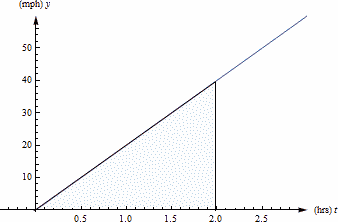
\includegraphics{images/image002.png}
\caption{}
\end{figure}

Each ordered pair \textbackslash{}((x, y)\textbackslash{}) specifies the
location of exactly one point, and the location of each point is given
by exactly one ordered pair \textbackslash{}((x, y)\textbackslash{}).
The \textbackslash{}(x\textbackslash{}) and
\textbackslash{}(y\textbackslash{}) values are the coordinates of the
point \textbackslash{}((x, y)\textbackslash{}).

The situation in three dimensions is very similar. In the 3-dimensional
rectangular coordinate system we have three coordinate axes that meet at
right angles, and three numbers, an ordered triple \textbackslash{}((x,
y, z)\textbackslash{}), are needed to specify the location of a point.

\begin{figure}
\centering
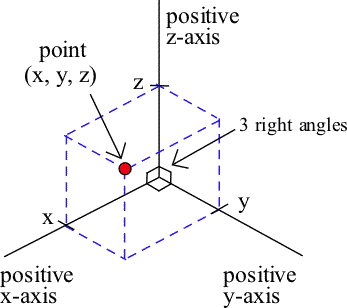
\includegraphics{images/image003.png}
\caption{}
\end{figure}

Each ordered triple \textbackslash{}((x, y, z)\textbackslash{})
specifies the location of exactly one point, and the location of each
point is given by exactly one ordered triple \textbackslash{}((x, y,
z)\textbackslash{}). The \textbackslash{}(x\textbackslash{}),
\textbackslash{}(y\textbackslash{}), and
\textbackslash{}(z\textbackslash{}) values are the coordinates of the
point \textbackslash{}((x, y, z)\textbackslash{}). The figure below
shows the location of the point (4, 2, 3).

\begin{figure}
\centering
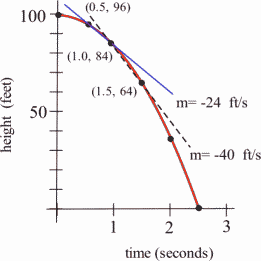
\includegraphics{images/image004.png}
\caption{}
\end{figure}

Typically we use a right-hand orientation. To see what this means,
imagine your right hand in front hand in front of you with the palm
toward your face, your thumb pointing up, you index finger straight out,
and your next finger toward your face (and the two bottom fingers bent
into the palm). Then, in the right hand coordinate system, your thumb
points along the positive \textbackslash{}(z\textbackslash{})-axis, your
index finger along the positive
\textbackslash{}(x\textbackslash{})-axis, and the other finger along the
positive \textbackslash{}(y\textbackslash{})-axis.

\begin{figure}
\centering
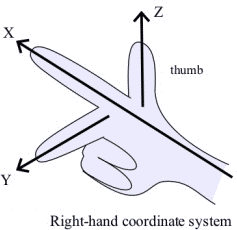
\includegraphics{images/image005.png}
\caption{}
\end{figure}

Other orientations of the axes are possible and valid (with appropriate
labeling), but the right-hand system is the most common orientation and
is the one we will generally use. If another orientation is used, then
the axes will be explicitly labeled.

Each ordered triple \textbackslash{}((x, y, z)\textbackslash{})
specifies the location of a single point, and this location point can be
plotted by locating the point \textbackslash{}((x, y,
0)\textbackslash{}) on the \textbackslash{}(xy\textbackslash{})-plane
and then going up \textbackslash{}(z\textbackslash{}) units (the red
path in the figure below).

\begin{figure}
\centering
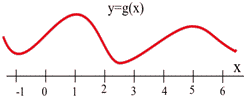
\includegraphics{images/image006.png}
\caption{}
\end{figure}

We could also get to the same \textbackslash{}((x, y,
z)\textbackslash{}) point in other ways. For instance, we could start by
finding the point \textbackslash{}((x, 0, z)\textbackslash{}) on the
\textbackslash{}(xz\textbackslash{})-plane and then going
\textbackslash{}(y\textbackslash{}) units parallel to the
\textbackslash{}(y\textbackslash{})-axis, or by finding
\textbackslash{}((0, y, z)\textbackslash{}) on the
\textbackslash{}(yz\textbackslash{})-plane and then going
\textbackslash{}(x\textbackslash{}) units parallel to the
\textbackslash{}(x\textbackslash{})-axis (the blue path in the figure
above).

\hypertarget{example-6}{%
\paragraph{Example 6}\label{example-6}}

Plot the locations of the points

\begin{itemize}
\tightlist
\item
  \textbackslash{}( P=(0,3,4) \textbackslash{}),
\item
  \textbackslash{}( Q=(2,0,4) \textbackslash{}),
\item
  \textbackslash{}( R=(1,4,0) \textbackslash{}),
\item
  \textbackslash{}( S=(3,2,1) \textbackslash{}), and
\item
  \textbackslash{}( T=(-1,2,1) \textbackslash{}).
\end{itemize}

The points are shown below.

\begin{figure}
\centering
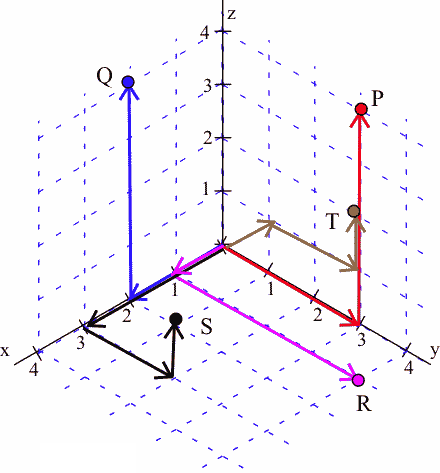
\includegraphics{images/image007.png}
\caption{}
\end{figure}

Once we can locate points, we can begin to consider the graphs of
various collections of points. By the graph of ``\textbackslash{}(z =
2\textbackslash{})'' we mean the collection of all points
\textbackslash{}((x, y, z)\textbackslash{}) which have the form
``\textbackslash{}((x, y, 2)\textbackslash{})''. Since no condition is
imposed on the \textbackslash{}(x\textbackslash{}) and
\textbackslash{}(y\textbackslash{}) variables, they take all possible
values. The graph of \textbackslash{}(z = 2\textbackslash{}) is a plane
parallel to the \textbackslash{}(xy\textbackslash{})-plane and 2 units
above the \textbackslash{}(xy\textbackslash{})-plane. Similarly, the
graph of \textbackslash{}(y = 3\textbackslash{}) is a plane parallel to
the \textbackslash{}(xz\textbackslash{})-plane, and \textbackslash{}(x =
4\textbackslash{}) is a plane parallel to the
\textbackslash{}(yz\textbackslash{})-plane. (Note: The planes have been
drawn as rectangles, but they actually extend infinitely far.)

\begin{figure}
\centering
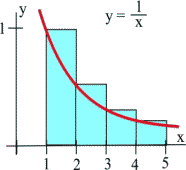
\includegraphics{images/image008.png}
\caption{}
\end{figure}

To view this video please enable JavaScript, and consider upgrading to a
web browser that \href{http://videojs.com/html5-video-support/}{supports
HTML5 video}

\hypertarget{distance-between-points}{%
\subsubsection{Distance Between Points}\label{distance-between-points}}

In two dimensions we can think of the distance between points as the
length of the hypotenuse of a right triangle, and that leads to the
Pythagorean formula: \textbackslash{}{[}
\textbackslash{}text\{distance\}=\textbackslash{}sqrt\{\textbackslash{}Delta
x\^{}2+\textbackslash{}Delta y\^{}2\}. \textbackslash{}{]}

\begin{figure}
\centering
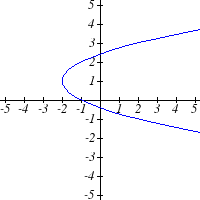
\includegraphics{images/image010.png}
\caption{}
\end{figure}

In three dimensions we can also think of the distance between points as
the length of the hypotenuse of a right triangle.

\begin{figure}
\centering
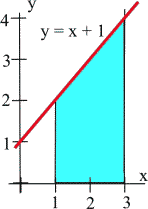
\includegraphics{images/image011.png}
\caption{}
\end{figure}

In this situation the calculations may appear more complicated, but they
are straightforward and the final formula is what we hope it would be
given the 2-dimensional formula: \textbackslash{}{[}
\textbackslash{}begin\{align*\} \textbackslash{}text\{distance\}\^{}2=\&
\textbackslash{}text\{base\}\^{}2+\textbackslash{}text\{height\}\^{}2
\textbackslash{}\textbackslash{} =\&
\textbackslash{}left(\textbackslash{}sqrt\{\textbackslash{}Delta
x\^{}2+\textbackslash{}Delta
y\^{}2\}\textbackslash{}right)\^{}2+\textbackslash{}Delta z\^{}2
\textbackslash{}\textbackslash{} =\& \textbackslash{}Delta
x\^{}2+\textbackslash{}Delta y\^{}2+\textbackslash{}Delta z\^{}2
\textbackslash{}end\{align*\} \textbackslash{}{]} so \textbackslash{}{[}
\textbackslash{}text\{distance\}=\textbackslash{}sqrt\{\textbackslash{}Delta
x\^{}2+\textbackslash{}Delta y\^{}2+\textbackslash{}Delta z\^{}2\}.
\textbackslash{}{]}

\hypertarget{distance-in-3-dimensions}{%
\paragraph{Distance in 3-Dimensions}\label{distance-in-3-dimensions}}

If \textbackslash{}(P = (x\_1 , y\_1 , z\_1 )\textbackslash{}) and
\textbackslash{}(Q = (x\_2 , y\_2 , z\_2 )\textbackslash{}) are points
in space, then the distance between \textbackslash{}(P\textbackslash{})
and \textbackslash{}(Q\textbackslash{}) is \textbackslash{}{[}
\textbackslash{}begin\{align*\} \textbackslash{}text\{distance\}=\&
\textbackslash{}sqrt\{\textbackslash{}Delta x\^{}2+\textbackslash{}Delta
y\^{}2+\textbackslash{}Delta z\^{}2\} \textbackslash{}\textbackslash{}
=\&
\textbackslash{}sqrt\{\textbackslash{}left(x\_2-x\_1\textbackslash{}right)\^{}2+\textbackslash{}left(y\_2-y\_1\textbackslash{}right)\^{}2+\textbackslash{}left(z\_2-z\_1\textbackslash{}right)\^{}2\}
\textbackslash{}end\{align*\} \textbackslash{}{]}

The 3-dimensional pattern is very similar to the 2-dimensional pattern
with the additional piece \textbackslash{}( \textbackslash{}Delta z\^{}2
\textbackslash{}).

\hypertarget{example-7}{%
\paragraph{Example 7}\label{example-7}}

Find the distances between points \textbackslash{}(A = (1, 2,
3)\textbackslash{}) and \textbackslash{}(B = (7, 5,
--3)\textbackslash{}).

\textbackslash{}{[}
\textbackslash{}text\{Dist\}(A,B)=\textbackslash{}sqrt\{6\^{}2+3\^{}2+(-6)\^{}2\}=\textbackslash{}sqrt\{36+9+36\}=\textbackslash{}sqrt\{81\}=9.
\textbackslash{}{]}

In two dimensions, the set of points at a fixed distance from a given
point is a circle, and we used the distance formula to determine
equations describing circles: the circle with center (2, 3) and radius 5
is given by \textbackslash{}((x--2)\^{}2 + (y--3)\^{}2 =
5\^{}2\textbackslash{}) or \textbackslash{}(x\^{}2 + y\^{}2 -- 4x -- 6y
= 12\textbackslash{}).

\begin{figure}
\centering
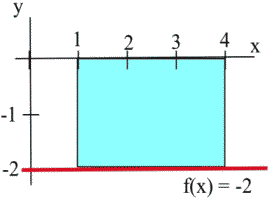
\includegraphics{images/image012.png}
\caption{}
\end{figure}

The same ideas work for spheres in three dimensions.

\hypertarget{spheres}{%
\paragraph{Spheres}\label{spheres}}

The set of points \textbackslash{}((x, y, z)\textbackslash{}) at a fixed
distance \textbackslash{}(r\textbackslash{}) from a point
\textbackslash{}((a, b, c)\textbackslash{}) is a sphere with center
\textbackslash{}((a, b, c)\textbackslash{}) and radius
\textbackslash{}(r\textbackslash{}).

\begin{figure}
\centering
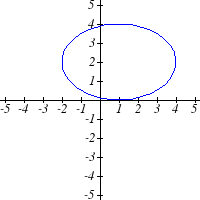
\includegraphics{images/image013.png}
\caption{}
\end{figure}

The sphere is given by the equation \textbackslash{}{[}
(x-a)\^{}2+(y-b)\^{}2+(z-c)\^{}2=r\^{}2. \textbackslash{}{]}

To view this video please enable JavaScript, and consider upgrading to a
web browser that \href{http://videojs.com/html5-video-support/}{supports
HTML5 video}

\hypertarget{example-8}{%
\paragraph{Example 8}\label{example-8}}

Write the equations of a sphere with center (2, -3, 4) and radius 3.

The equation is \textbackslash{}{[}
(x-2)\^{}2+(y+3)\^{}2+(z-4)\^{}2=3\^{}2. \textbackslash{}{]}

Now suppose that we want to graph a surface. We can think of each input
\textbackslash{}((x,y)\textbackslash{}) as a location on the plane, and
plot the point \textbackslash{}(f(x,y)\textbackslash{}) units above that
point. Graphing that can be challenging. We have a few options:

\begin{enumerate}
\item
  Use a computer program (such as GeoGebra or Mathematica) to draw
  beautiful perspective drawings.

  \begin{figure}
  \centering
  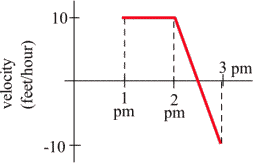
\includegraphics{images/image014.png}
  \caption{}
  \end{figure}

  If such a program is available, then this is usually the most accurate
  option.
\item
  Try to draw a perspective drawing by hand. This is very challenging,
  and usually not worth the effort.
\item
  Use level curves to draw \textbf{contour diagrams} (or \textbf{contour
  maps}), which is the approach we'll focus on here. A contour diagram
  is like a topographical map -- points with the same elevation
  (outputs) are connected with curves. Each particular output is called
  a \emph{level}, and these curves are called \emph{level curves} or
  \emph{contours}. The closer the curves are to each other, the steeper
  that section of the surface. Topographical maps give hikers
  information about elevation, steep and shallow grades, peaks and
  valleys. Contour diagrams give us the same kind of information about a
  function.
\end{enumerate}

Below is a contour diagram of the same surface shown in above. The level
curves are graphs in the \textbackslash{}(xy\textbackslash{})-plane of
curves \textbackslash{}(f(x, y) = c\textbackslash{}) for various
constants \textbackslash{}(c\textbackslash{}).

\begin{figure}
\centering
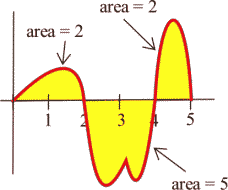
\includegraphics{images/image015.png}
\caption{}
\end{figure}

Each of the squares corresponds to one of the bumps on the surface. If
the contours are positive, as highlighted below, the bump is above the
\textbackslash{}(xy\textbackslash{})-plane. If the contours are
negative, the bump extends below the
\textbackslash{}(xy\textbackslash{})-plane.

\begin{figure}
\centering
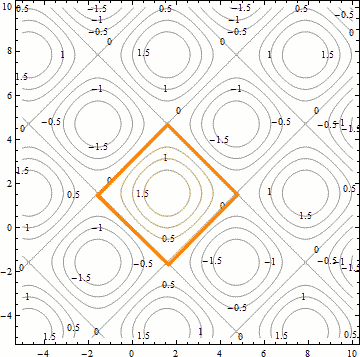
\includegraphics{images/image016.png}
\caption{}
\end{figure}

Everywhere on the crisscrossed pattern of diagonal lines, the height of
the surface is 0, so the surface is on the
\textbackslash{}(xy\textbackslash{})-plane. This is a feature that we
wouldn't necessarily have seen when we looked at the perspective
drawing. Contour maps can help us see features of the surface that the
3-dimensional graph doesn't show.

\begin{figure}
\centering
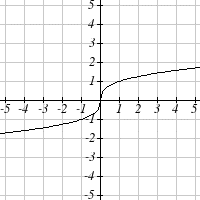
\includegraphics{images/image017.png}
\caption{}
\end{figure}

To better understand contour diagrams, suppose we had a table of
elevation data. We could graph this by plotting the height at each point
and connecting the dots with smooth curves, which would result in the
something like the graph shown.

\begin{figure}
\centering
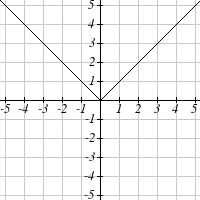
\includegraphics{images/image018.png}
\caption{}
\end{figure}

If we ``slice'' the surface above with the plane \textbackslash{}(z =
8\textbackslash{}), the points where the plane cuts the surface are
those points where the elevation of the surface is 8 units above the
\textbackslash{}(xy\textbackslash{})-plane. The figure below shows the
surface being sliced by the planes \textbackslash{}(z =
8\textbackslash{}) and \textbackslash{}(z = 4\textbackslash{}). Slicing
the surface at different elevations and sketching the curves where the
plane intersects the surface results in the second graph below.

\begin{figure}
\centering
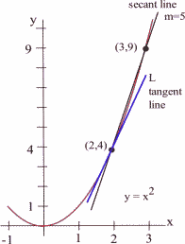
\includegraphics{images/image020.png}
\caption{}
\end{figure}

If we move all of those curves to the xy--plane (or, equivalently, view
them from directly overhead), the result is a 2-dimensional graph of the
level curves of the original surface. This is the contour diagram.

\begin{figure}
\centering
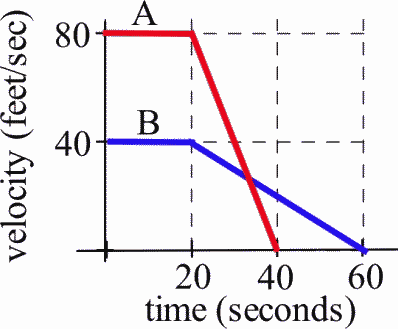
\includegraphics{images/image022.png}
\caption{}
\end{figure}

To view this video please enable JavaScript, and consider upgrading to a
web browser that \href{http://videojs.com/html5-video-support/}{supports
HTML5 video}

\hypertarget{example-9}{%
\paragraph{Example 9}\label{example-9}}

Create a contour diagram for our car rental example with cost function
\textbackslash{}( C(d,m)=40d+0.15m \textbackslash{}). Draw curves for
when the cost is 0, 100, 200, 300, and 400.

We'll set \textbackslash{}( C(d,m)=40d+0.15m=c \textbackslash{}) for
\textbackslash{}(c =\textbackslash{}) 0, 100, 200, 300, and 400 and draw
the curves in the \textbackslash{}(dm\textbackslash{})-plane.

The first coordinate of the ordered pair is
\textbackslash{}(d\textbackslash{}), so the
\textbackslash{}(d\textbackslash{})-axis will be horizontal; the
\textbackslash{}(m\textbackslash{})-axis will be vertical. Remember that
the domain for this function is really just where \textbackslash{}(d
\textbackslash{}geq 0\textbackslash{}) and \textbackslash{}(m
\textbackslash{}geq 0\textbackslash{}), so we will only draw the curves
in the first quadrant.

When \textbackslash{}( c=0 \textbackslash{}): \textbackslash{}{[}
\textbackslash{}begin\{align*\} C(d,m)=\& 40d+0.15m=0
\textbackslash{}\textbackslash{} 0.15m=\& -40d
\textbackslash{}\textbackslash{} m=\&
-\textbackslash{}frac\{40\}\{0.15\}d\textbackslash{}approx -267d
\textbackslash{}end\{align*\} \textbackslash{}{]}

This is the equation of a line, with slope about -267, passing through
the origin. Because of the domain restrictions, the ``curve'' we will
draw for this level is simply the origin. Putting this back into the car
rental context, the only point where we pay \$0 for renting the car is
when we rent the car for 0 days and drive it 0 miles -- that is, if we
don't rent it at all.

When \textbackslash{}( c=100 \textbackslash{}): \textbackslash{}{[}
\textbackslash{}begin\{align*\} C(d,m)=\& 40d+0.15m=100
\textbackslash{}\textbackslash{} 0.15m=\& -40d+100
\textbackslash{}\textbackslash{} m=\&
-\textbackslash{}frac\{40\}\{0.15\}d+\textbackslash{}frac\{100\}\{0.15\}\textbackslash{}approx
-267d+667 \textbackslash{}end\{align*\} \textbackslash{}{]}

This is the equation of a line, with slope about -267, and
\textbackslash{}(d\textbackslash{})-intercept of about 667. This section
of this line that lies in the first quadrant is shown with 100 labeling
it.

Putting this into context, any point on that line represents a
\textbackslash{}((d, m)\textbackslash{}) combination of days and miles
that will make the cost exactly \$100. So, for example -- if we rent the
car for 0 days and drive it 667 miles, it will cost us \$100. If we rent
the car for 2.5 days and don't drive any miles, it will cost us \$100.

We continue for \textbackslash{}(c =\textbackslash{}) 200, 300, and 400
and sketch the curves in the plane, resulting in the contour diagram
shown to the right.

\begin{figure}
\centering
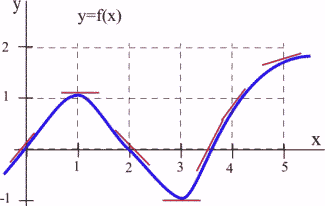
\includegraphics{images/image023.png}
\caption{}
\end{figure}

\hypertarget{example-10}{%
\paragraph{Example 10}\label{example-10}}

The contour diagram for the cost
\textbackslash{}(C(d,m)\textbackslash{}) in dollars for renting a car
for \textbackslash{}(d\textbackslash{}) days and driving it
\textbackslash{}(m\textbackslash{}) miles is shown in the previous
example. Use the diagram to answer the following questions.

\begin{enumerate}
\tightlist
\item
  What is the cost of renting a car for 3 days and driving it 200 miles?
\item
  What is \textbackslash{}(C(100, 4)\textbackslash{})? What is
  \textbackslash{}(C(4, 100)\textbackslash{})?
\item
  Suppose we rent the car for 3 days. Is
  \textbackslash{}(C\textbackslash{}) an increasing function of miles?
\end{enumerate}

\begin{enumerate}
\item
  The point (3, 200) is between contours on this graph, so we can't get
  an exact answer for \textbackslash{}(C(3, 200)\textbackslash{}). (But
  it's typical for a graph that we would have to estimate). It looks to
  me as if (3, 200) is halfway between the 100 and the 200 contours, so
  let's estimate that \textbackslash{}(C(3, 200)\textbackslash{}) is
  about \$150.

  Estimates from the graph are necessarily very rough. The graph only
  shows a little information (in this way, a contour diagram is like a
  table), so we have to extrapolate in between. But for most graphs, we
  don't actually know what happens between the contours. All we know for
  sure is that the output at (3, 200) is between the two levels we see.
  For this car rental example, we also know a formula, and my table
  showed this particular input, so we have other ways to get a better
  answer.
\item
  We can't find (100, 4) on this diagram, so we can't make an estimate
  of \textbackslash{}(C(100, 4)\textbackslash{}) from this graph. (4,
  100) lies between the contours for 100 and 200. It looks closer to
  200, so let's estimate that \textbackslash{}(C(4,
  100)\textbackslash{}) is about \$180.
\item
  If we fix \textbackslash{}(d = 3\textbackslash{}), we get a vertical
  line. What happens as \textbackslash{}(m\textbackslash{}) increases on
  this vertical line? As \textbackslash{}(m\textbackslash{}) increases,
  the function values shown on the contours increase, so
  \textbackslash{}(C\textbackslash{}) appears to be an increasing
  function of miles.

  \begin{figure}
  \centering
  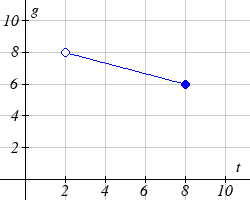
\includegraphics{images/image024.png}
  \caption{}
  \end{figure}
\end{enumerate}

\hypertarget{example-11}{%
\paragraph{Example 11}\label{example-11}}

Here is a contour diagram for a function
\textbackslash{}(g(x,y)\textbackslash{}).

\begin{figure}
\centering
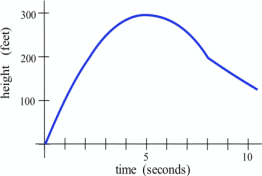
\includegraphics{images/image025.png}
\caption{}
\end{figure}

Use the diagram to answer the following questions:

\begin{enumerate}
\tightlist
\item
  What is \textbackslash{}(g(3, 5)\textbackslash{})?
\item
  What is the highest point shown on the diagram? What is the lowest
  point shown?
\item
  If you start at (3, 5) and head in the positive
  \textbackslash{}(x\textbackslash{}) direction, do you go uphill or
  downhill first?
\end{enumerate}

\begin{enumerate}
\item
  \textbackslash{}(g(3, 5)\textbackslash{}) is 0.6. We can tell because
  the point is right on one of the contours, as illustrated in the image
  below.

  \begin{figure}
  \centering
  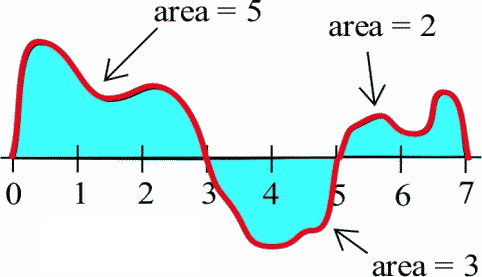
\includegraphics{images/image026.png}
  \caption{}
  \end{figure}
\item
  The highest contour shown is 0.9, and there would be a contour for 1.0
  if the surface had ever got that high. However, the height seems to be
  increasing as we move in toward the center, so it appears that
  \textbackslash{}(g\textbackslash{}) gets to nearly 1 in the center.
  The lowest contour is 0.1. But again, we will guess that the height
  continues to decrease, so it appears that
  \textbackslash{}(g\textbackslash{}) is nearly 0 around the outside.
\item
  Starting at the point (3, 5, 0.6) on the surface and traveling to the
  right along the horizontal line shown in the previous part, we would
  cross the contour for 0.7 next. So the function increases first (we go
  uphill), and then decreases again.
\end{enumerate}

Again, remember that we don't really know what happens between the
contours. All we can do is estimate from the information in the graph.

\hypertarget{example-12}{%
\paragraph{Example 12}\label{example-12}}

Here is a contour diagram for a function
\textbackslash{}(F(x,y)\textbackslash{}).

\begin{figure}
\centering
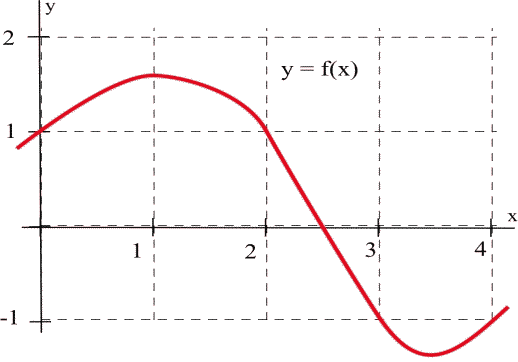
\includegraphics{images/image027.png}
\caption{}
\end{figure}

\begin{enumerate}
\tightlist
\item
  Describe the shape of the surface.
\item
  Suppose you travel along the surface in the positive
  \textbackslash{}(y\textbackslash{})-direction, starting on the surface
  at the point above (or below) the point \textbackslash{}((x, y) = (-1,
  1)\textbackslash{}). Describe your journey.
\end{enumerate}

\begin{enumerate}
\item
  The surface is bumpy, with regularly spaced oval bumps. Notice that
  some of the bumps go up (positive contours), but others go down.
  Between the bumps, there are horizontal lines that are completely
  level, with an elevation of 0.
\item
  It looks as if \textbackslash{}(F(-1,1)\textbackslash{}) is about 3.
  As we head in the positive
  \textbackslash{}(y\textbackslash{})-direction along the line shown
  below, we first go uphill, nearly to 4, then we start going downhill.
  As we keep going north, we keep descending, going into the dip, until
  nearly -4. We're starting to go uphill again just as we leave the
  graph.

  \begin{figure}
  \centering
  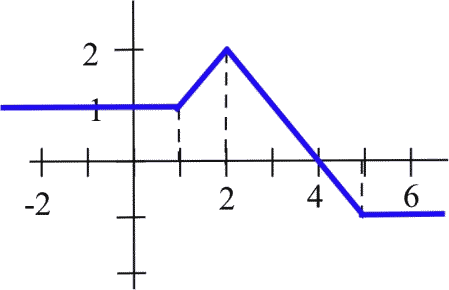
\includegraphics{images/image028.png}
  \caption{}
  \end{figure}
\end{enumerate}

What happens if you have a function of more than two variables? Its
graph will be a \emph{hyper-surface}. For example, the graph of a
function of four variables will be a hyper-surface in 5-dimensional
space. This is very difficult (impossible for most of us) to visualize.
Even the contours are hard to visualize -- instead of curves in the
plane, they're hyper-surfaces in 4-dimensional space. So if you have
more than two variables, the graph isn't usually very useful.

\hypertarget{functions-of-two-real-life-variables}{%
\subsection{Functions of Two Real-Life
Variables}\label{functions-of-two-real-life-variables}}

\hypertarget{complementary-goods-and-substitute-goods}{%
\subsubsection{Complementary Goods and Substitute
Goods}\label{complementary-goods-and-substitute-goods}}

The demand for some pairs of goods have a relationship, where the
quantity demanded for one product depends somehow on the prices for both

\hypertarget{complementary-goods}{%
\paragraph{Complementary Goods}\label{complementary-goods}}

Two goods are \textbf{complementary} if an increase in the price of
either decreases the demand for both.

Examples:

\begin{itemize}
\tightlist
\item
  The demand for cars depends on both the price for cars and the price
  of gasoline.
\item
  The demand for hot dog buns depends on both the price for the buns and
  the price for the hot dogs.
\end{itemize}

\hypertarget{substitute-goods}{%
\paragraph{Substitute Goods}\label{substitute-goods}}

Two goods are \textbf{substitutes} if an increase in the price of one
increases the demand for the other.

Example:

\begin{itemize}
\tightlist
\item
  The demand for Brand A depends on its price and also on the price of
  its main competitor Brand B. If the Brand B raises its price,
  consumers will switch brands (substitute) and demand for Brand A will
  increase.
\end{itemize}

Think brands of soft drinks, detergent, or paper towels. A traditional
example is coffee and tea: the idea is that consumers are simply looking
for a hot drink and they'll buy whatever is cheaper. But this has always
seemed fishy to me -- I've never met any coffee- or tea-drinkers who
would happily switch.

These demand functions are functions of two variables.

\hypertarget{example-13}{%
\paragraph{Example 13}\label{example-13}}

The demand functions for two products are given below.
\textbackslash{}(p\_1\textbackslash{}),
\textbackslash{}(p\_2\textbackslash{}),
\textbackslash{}(q\_1\textbackslash{}), and
\textbackslash{}(q\_2\textbackslash{}) are the prices (in dollars) and
quantities for Products 1 and 2: \textbackslash{}{[}
\textbackslash{}begin\{align*\} q\_1=\& 200-3p\_1-p\_2
\textbackslash{}\textbackslash{} q\_2=\& 150-p\_1-2p\_2
\textbackslash{}end\{align*\} \textbackslash{}{]}

Are these two products complementary goods or substitute goods? What is
the quantity demanded for each when the price for Product 1 is \$20 per
item and the price for Product 2 is \$30 per item?

These products are complementary: an increase in either price decreases
both demands. You can see that because the coefficients are both
negative in each demand function.

When \textbackslash{}(p\_1 = 20\textbackslash{}) and
\textbackslash{}(p\_2 = 30\textbackslash{}), we have \textbackslash{}{[}
\textbackslash{}begin\{align*\} q\_1=\& 200-3(20)-(30)=110
\textbackslash{}\textbackslash{} q\_2=\& 150-(20)-2(30)=70
\textbackslash{}end\{align*\} \textbackslash{}{]} So 110 units are
demanded for Product 1 and 70 units are demanded for Product 2 when the
price for Product 1 is \$20 per item and the price for Product 2 is \$30
per item.

\hypertarget{cobb-douglas-production-function}{%
\subsubsection{Cobb-Douglas Production
Function}\label{cobb-douglas-production-function}}

Production functions are used to model the total output of a firm for a
variety of inputs (doesn't this sound like a function of several
variables?). One example is a Cobb-Douglas Production function:
\textbackslash{}{[}
P=AL\^{}\{\textbackslash{}alpha\}K\^{}\{\textbackslash{}beta\}
\textbackslash{}{]}

In this function \textbackslash{}(P\textbackslash{}) is the total
production, \textbackslash{}(A\textbackslash{}) is a constant,
\textbackslash{}( \textbackslash{}alpha \textbackslash{}) and
\textbackslash{}( \textbackslash{}beta \textbackslash{}) are constants
between 0 and 1, \textbackslash{}(L\textbackslash{}) is the labor force,
and \textbackslash{}(K\textbackslash{}) is the capital expenditure. (The
units must be massaged well.)

You can read more about Cobb-Douglas Production functions at
\url{http://en.wikipedia.org/wiki/Cobb-Douglas}. You can read about
other kinds of production functions at
\url{http://en.wikipedia.org/wiki/Production_function}.

\begin{longtable}[]{@{}ll@{}}
\toprule
\endhead
\href{../chapter3/section3-8.php}{← Previous Section} &
\href{section4-2.php}{Next Section →}\tabularnewline
\bottomrule
\end{longtable}
